\begin{frame}{Starting Point: The NSAK Framework}
    \framesubtitle{Established in the predecessor project (Project 2)}

    \begin{columns}[T,onlytextwidth]
        \begin{column}{0.5\textwidth}
            \vspace*{0.8cm}
            \textbf{A modular, open-source network security}\\\textbf{framework}

            \vspace{0.6em}
            Built around four reusable resource types:
            \vspace{0.4em}
            \begin{itemize}
                \item[\faServer] \textbf{Device} \textit{\scriptsize execution host at a network position}
                \item[\faNetworkWired] \textbf{Environment} \textit{\scriptsize target network topology}
                \item[\faLayerGroup] \textbf{Scenario} \textit{\scriptsize a red/blue team use case}
                \item[\faCogs] \textbf{Drill} \textit{\scriptsize reusable building block}
            \end{itemize}
        \end{column}

        \begin{column}{0.5\textwidth}
            \centering
            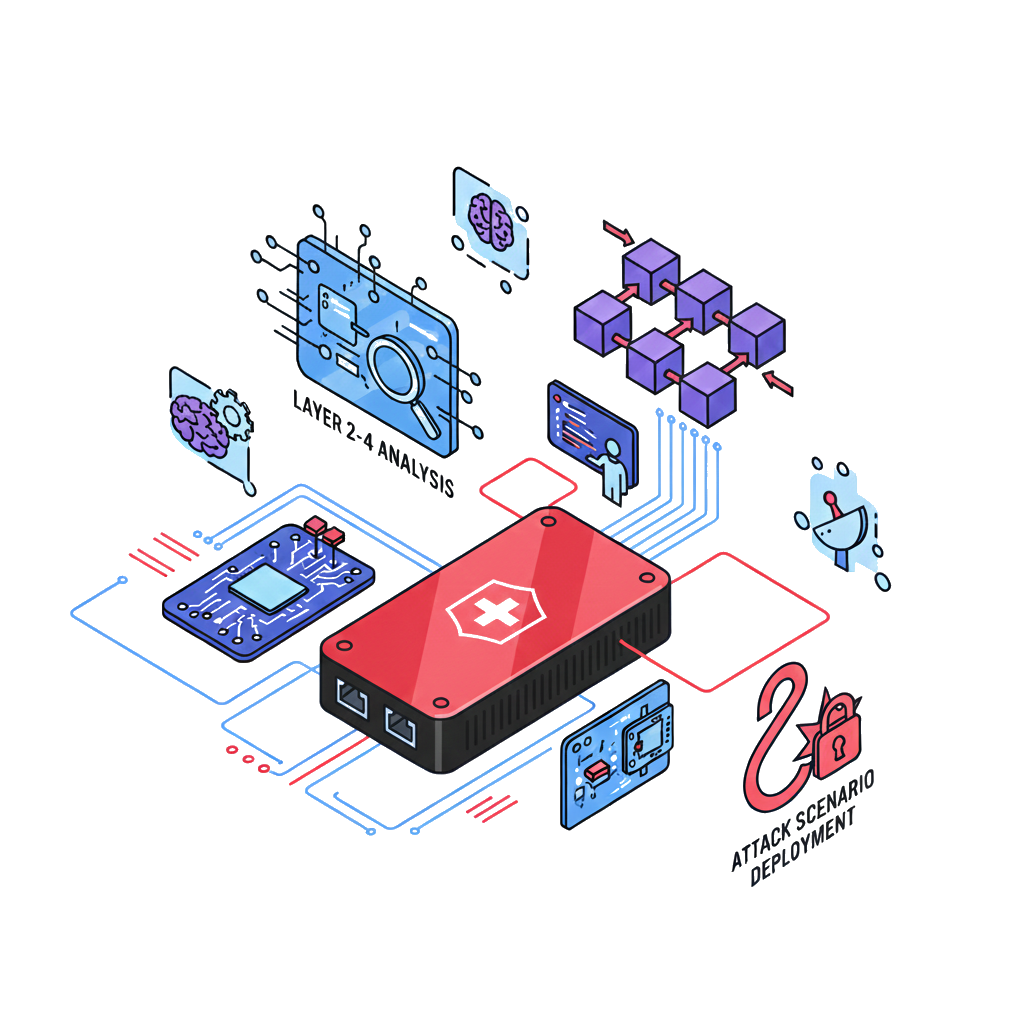
\includegraphics[width=0.9\linewidth]{assets/swiss-army-nsak-transparent}
        \end{column}
    \end{columns}
\end{frame}
\begin{frame}{Hypothesis and Research Questions}
    \framesubtitle{From static scenarios to agentic AI}
    \uncover<1->{
        \begin{block}{Hypothesis}

            \small
            Integrating \textbf{agentic AI} into NSAK improves \textbf{adaptability, flexibility} and
            \textbf{automation} over static scenarios, while \textbf{lowering the operator's required expertise}
            to interpret results and plan follow-up steps.

        \end{block}
    }
\end{frame}
\begin{frame}{Layered Architecture}
    \framesubtitle{system-diagram}

        \centering
        \includesvg[width=\linewidth,height=0.78\textheight,keepaspectratio]{assets/diagram/system-container}
        \label{fig:system-container}
\end{frame}
